\chapter*{Введение}
\addcontentsline{toc}{chapter}{Введение}

    Одна из задач в области искусственного интеллекта~--- задача планирования.
 Планированием называется процесс выработки последовательности действий, позволяющей достичь цели \cite{norwig-ai}.
 Задача планирования часто возникает у агентов, которым нужно найти последовательность действий, выполнив которые он достигнет некоторой своей цели.
 Агентом можно назвать все, что воспринимает свою среду с помощью некоторых датчиков и воздействует на нее с помощью некоторых механизмов.
 Примерами использования планирования может служить следующее: планирование управлением механическими приводами робота-мусоросборника, планирование распределения транспортных средств для перевозок различных видов топлива и сырья на нефтеперерабатывающем заводе.
 
    Контекст задачи планирования, модель мира, в котором возникает задача,  называется предметной областью.
    
    %В 1971 году для представления знаний о предметных областях был разработан формальный текстовый язык STRIPS\footnote{STanford Research Institute Problem Solver}\cite{strips}.
 Для описания знаний систем планирования выделяют три основных понятия~--- \textit{состояние среды} (мира), \textit{действие} (механизмы воздействия на среду), \textit{цель} (утверждение о целевом состоянии мира).
 Состояния задаются в виде некоторого набора фактов об объектах и отношениях между ними, которые считаются истинными в этом состоянии.
 Действия задаются с использованием набора ограничений на состояние (предусловие), и набора положительных и отрицательных фактов (эффекты).
 \textit{Предусловие} должно выполняться для того, чтобы применение действия было допустимым в данном состоянии.
 \textit{Эффект} задает то, как меняется состояние при применении действия~--- положительные факты добавляются к состоянию, отрицательные~--- удаляются.
 \textit{Цель}, или целевое состояние, задается как набор ограничений, которые должны быть удовлетворены в данном состоянии.
 Для того, чтобы упростить описание состояний вводится гипотеза замкнутости мира, которая означает, что факты, не перечисленные в описании состояния, считаются ложными.
    
%В 1987 году был предложен язык ADL (Action Description Language, язык описания действий) похожий на STRIPS, но включающий в себя еще несколько дополнительных возможностей.
В 70-е годы появляются первые формальные текстовые языки для описания знаний систем планирования. Как попытка стандартизации этих языков в 1988 году появился полноценно используемый и в наше время язык PDDL\footnote{Planning Domain Definition Language~--- язык описания предметных областей и задач планирования}\cite{pddl3}. Он постепенно адаптировался и дополнялся, а уже в 1998 году PDDL стал языком международных соревнования по созданию планировщиков IPC\footnote{International Planing Competition}. 
На данный момент PDDL является стандартом де-факто для описания знаний систем планирования.

В современной программной инженерии широко используются объектные графические нотации для моделирования и спецификации программных систем. Массово применяется язык UML\footnote{Unified Modeling Language~--- унифицированный язык моделирования}\cite{rambo-uml2}. Составление UML-диаграмм стало неотъемлемой частью практики многих специалистов. Это стало причиной многих успешных попыток применять навыки работы с UML в области инженерии знаний. На международной конференции ICAPS~\footnote{International Conference on Automated Planning and Scheduling} из года в год делаются сообщения о новых проектах\cite{icaps-1, icaps-2}, базирующихся на использовании UML для представления знаний. В рамках этих проектов создаются инструменты, обеспечивающие специалистам по инженерии знаний возможность применять в своей работе UML. Распространяется подход, при котором инженер знаний описывает предметные области и условия задач планирования в виде UML-моделей, а затем генерирует по созданным моделям описания на языке PDDL. Отправным пунктом дипломной работы является желание дополнить указанный подход обратным преобразованием PDDL-описания в UML-модель. Дело в том, что за многие годы накоплено значительное количество описаний предметных областей и задач планирования (например, в архивах чемпионата IPC). При переходе инженеров знаний к использованию UML работа с архивами описаний упростится, если будет реализован перевод с PDDL на UML.

Исходя из сказанного выше, можно заключить, что тема дипломной работы актуальна, а её результаты имеют практическое значение.
На рис. \ref{img:scheme} показано место генератора, который планируется разработать в данной работе, в среде инженерии знаний системы планирования.
 
\begin{figure}[h]
    \center{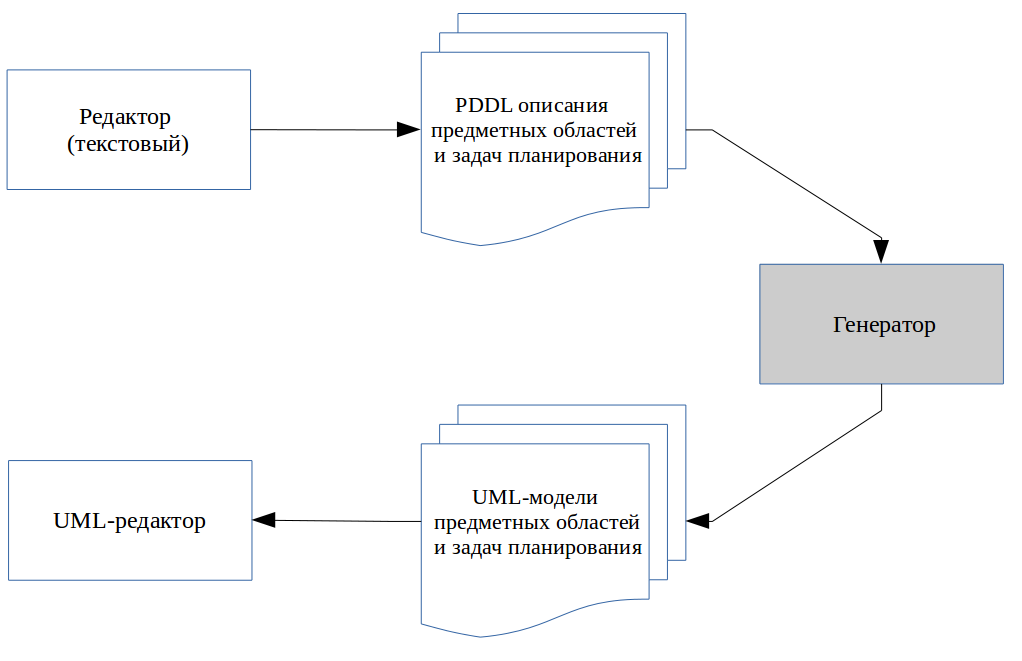
\includegraphics[width=0.8\linewidth]{scheme}}
    \caption{Генератор, обеспечивающий полноценную работу с архивными описаниями в рамках инженерии знаний с использованием UML}
    \label{img:scheme}
\end{figure}   
%В настоящее время большую популярность приобретают графические представления, основанные на объектных спецификациях.
%Для графического моделирования и удовлетворения нужд программной индустрии был разработан язык UML\footnote{Unified Modeling Language~--- унифицированный язык моделирования}\cite{rambo-uml2}, но его возможности оказались шире, поэтому он может быт использован и в других областях,например, в инженерии знаний для представления знаний систем планирования в виде UML-моделей. В настоящее время появляется большое количество людей, привыкших работать с такими графическими нотациями.

%В инженерии знаний все чаще используются графические нотации на основе объектных спецификаций, на международной конференции ICAPS~\footnote{International Conference on Automated Planning and Scheduling} делаются доклады\cite{icaps-1, icaps-2} по объектной инженерии знаний планировщиков и систем планирования. Если нужно получить план решения задачи, то знания, описанные UML-моделями, транслируются в PDDL и затем передаются планировщикам для нахождения плана. Но если со знаниями нужно делать что-то еще, то большое значение имеют возможности преобразования знаний и трансляции знаний в другие представления. Для работы со знаниями, представленными в виде UML-моделей, в этом направлении могут использоваться уже существующие в большом количестве различные стандарты и инструменты M2M и M2T. За прошедшее время на соревнованиях IPC накопились большие архивы задач, которые можно было бы перевести в UML-модели для более удобной работы с ними. Исходя из вышесказанного, можно заключить, что актуальна задача получения UML-представления знаний о предметных областях и задачах планирования по их текстовым описаниям на языке PDDL. 

%Для задания дополнительных ограничений на UML-модели может быть использован язык OCL\footnote{Object Constraint Language~--- язык объектных ограничений}\cite{ocl}.
% Для создания UML-моделей существует множество редакторов, что делает возможность задания знаний среды и задачи планирования в графическом представлении более привлекательной. 
%По этой теме на международной конференции ICAPS~\footnote{International Conference on Automated Planning and Scheduling} было представлено несколько докладов \cite{icaps-1, icaps-2}. 
    

%Поэтому в данной работе исследуется такая задача из области планирования, как преобразование представлений знаний систем планирования. 

\newpage